%%%%%%%%%%%%%%%%%%%%%%%%%%%%%%%%%%%%%%%%%%%%%%%%%%%%%%%%%%%%%%%%%%%%%%%%%%%%%%%%%%%%%%%%%%%%%
%%									Chapitre 4												%
%%%%%%%%%%%%%%%%%%%%%%%%%%%%%%%%%%%%%%%%%%%%%%%%%%%%%%%%%%%%%%%%%%%%%%%%%%%%%%%%%%%%%%%%%%%%%

\chapter{Is it optimal to group policyholders by age, gender, and seniority for BEL computations based on model points?}\label{Chapter6}
	\minitoc
	\newpage

%%%%%%%%%%%%%%%%%%%%%%%%%%%%%%%%%%%%%%%%%%%%%%%%%%%%%%%%%%%%%%%%%%%%%%%%%%%%%%%%%%%%%%%%%%%%%



% Début du chapitre
%\includepdfset{pagecommand=\thispagestyle{scrheadings}} % ajoute les numéros de page aux pdf importés
%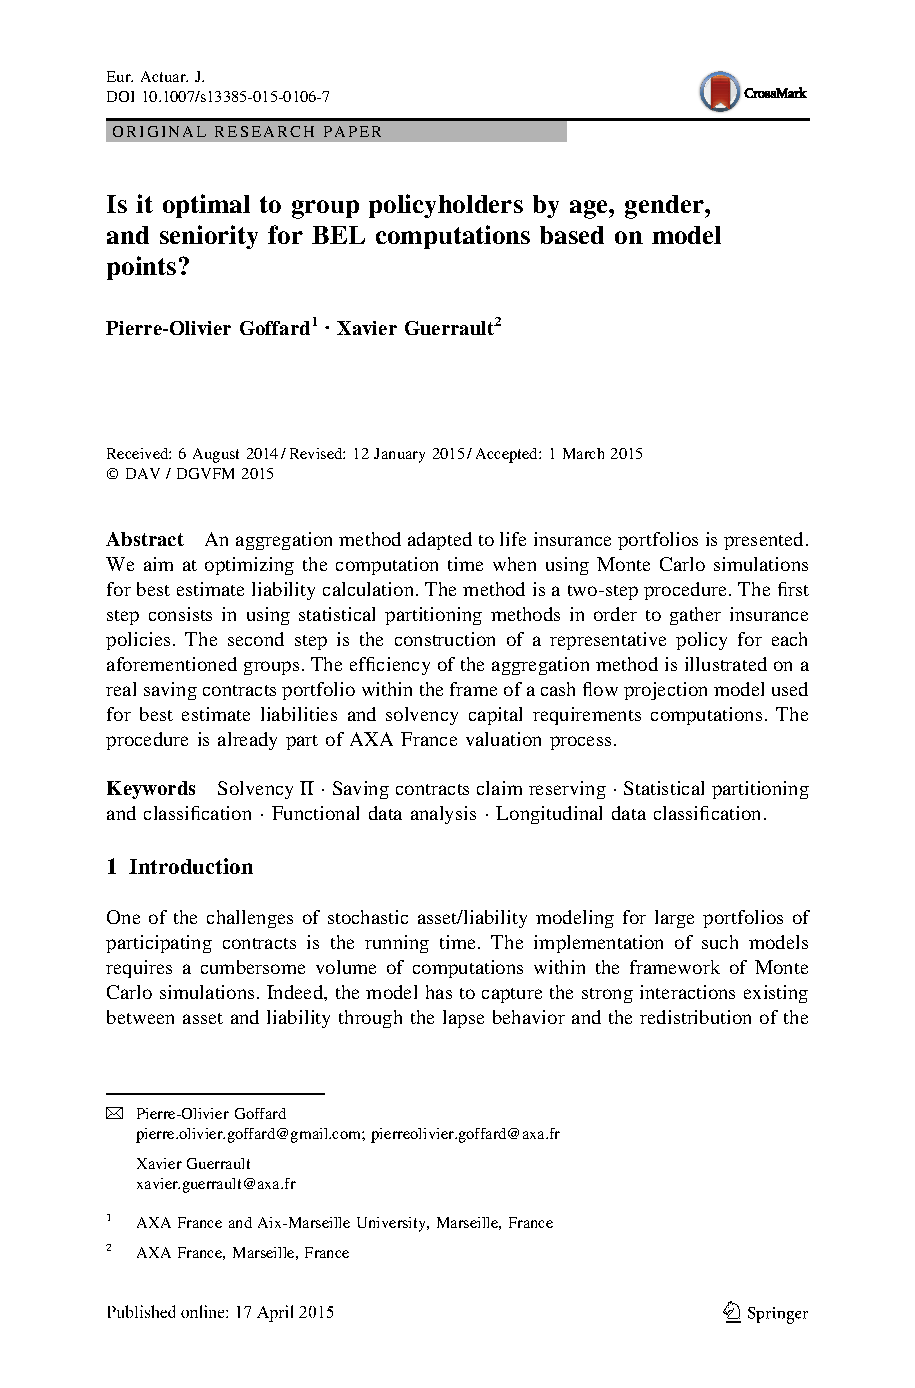
\includepdf[pages=-]{Chapitre6/GoffardGuerraultModelPointsEaJ2015.pdf}
\begin{center}
\Large{\underline{\textbf{Abstract}}}\\
\end{center}
An aggregation method adapted to life insurance portfolios is presented. We aim at optimizing the computation time when using Monte Carlo simulations for best estimate liability calculation. The method is a two-step procedure. The first step consists in using statistical partitioning methods in order to gather insurance policies. The second step is the construction of a representative policy for each aforementioned groups. The efficiency of the aggregation method is illustrated on a real saving contracts portfolio within the frame of a cash flow projection model used for best estimate liabilities and solvency capital requirements computations. The procedure is already part of AXA France valuation process.\\
\\
\textit{Keywords:} Solvency II, saving contracts claim reserving, statistical partitioning and classification, functional data analysis, longitudinal data classification. 
\section{Introduction}
One of the challenges of stochastic asset/liability modeling for large portfolios of participating contracts is the running time. The implementation of such models requires a cumbersome volume of computations within the framework of Monte Carlo simulations. Indeed, the model has to capture the strong interactions existing between asset and liability through the lapse behavior and the redistribution of the financial and technical result. For an overview we refer to Planchet et al. \citet{PlThJu11}. Using a stochastic asset/liability model to analyze large blocks of business is often too time consuming to be practical. Practitionners make compromises to tackle this issue.\\
\\
Grouping methods, which group policies into model cells and replace all policies in each groups with a representative policy, is the oldest form of modelling techniques. It has been advised in \citet{EIOPA} and is commonly used in practice due to its availability in commercial actuarial softwares such as MG-ALFA, GGY-Axis and TRICAST suite. In a recent PhD thesis \citet{Sa13}, representative portfolios have been drawn from a stratified sampling procedure over the initial portfolio. Computations are achieved on this smaller portfolio and the procedure is repeated to yield a final approximation. The idea  remains to reduce the computation time by reducing the number of model cells.\\
\\
Another idea consists in reducing the computation time for one policy. For instance one may think about reducing the number of economic scenarios. In \citet{DeLo09} an algorithm, inspired by importance sampling, is presented to select the most relevant financial scenarios in order to estimate quantiles of interest. Applications to the estimation of remote (but not extreme) quantiles can be found in \citet{ChDeLoMD11}, in addition to consistency results regarding the estimator. However, we are interested in the calculation of the value of Best Estimate Liabilities (BEL) for participating contracts, which are the probability weighted average of future cash flows taking into account the time value of money. Therefore, Planchet et al. \citet{NtPl12} presented a way to aggregate all the scenarios in a set of characteristic trajectories associated to a probability of occurence, well adapted to BEL computations. Another well-known modeling technique when dealing with financial sensitivities is the replicating portfolio method. As life insurance contracts share many features with derivative contracts, the idea of representing liabilities by a portfolio of financial products comes naturally. For an overview of the replicating portfolio method, we refer to \citet{Sc08,DeCh11}. We also want to mention the work of Planchet et al. \citet{BoPlJu12}, where an analytical approximation formula for best estimate valuation of saving contracts is derived. The approximation is based on the evaluation of a coefficient, which when applied to the mathematical reserve yields the BEL. We believe that the ways of dealing with computation time issues are not in competition, for instance a grouping method combined with an optimization of financial scenarios may yield great results.\\
\\
In this paper, we present a new grouping method and we focus on the calculation of the value of Best Estimate Liabilities (BEL) for participating contracts via an asset/liability model. This work has been motivated by the revision of the valuation process in AXA France to be compliant with Solvency II. The aggregation method must meet many practical requirements such as easy implementation and understanding, applicability to the whole life insurance portfolio and good empirical and theoretical justification. We believe that many insurance companies face computation time problems, and this paper may help practionners to solve it. In Section 2, we give a description of the cash flow projection model being used. In Section 3, we describe a statistical based way to group policies, followed by procedures to construct the representative policy. Section 4 illustrates the efficiency of the method on a portfolio of saving contracts on the French market.
\section{Cash flows projection models and best estimate liabilities assessment}
We consider a classical asset-liability model to project the statutory balance sheet and compute mathematical reserves for saving contracts. The settings and notations are closed to those in \citet{BoPlJu12}. Consider a saving contract with surrender value $SV(0)$ at time $t=0$, the surrender value at time $t$ is defined as
\begin{equation}\label{SV}
SV(t)=SV(0)\times exp\left(\int^{t}_{0}r_{a}(s)ds\right),
\end{equation}
where $r_{a}$ denotes the instantaneous accumulation rate (including any guaranteed rate) modeled by a stochastic process. We are interested in the present surrender value at time $t$, we need therefore to add a discount factor in order to define the Present Surrender Value
\begin{eqnarray}
PSV(t)&=&SV(t)\times exp\left(-\int^{t}_{0}r_{\delta}(s)ds\right)\nonumber\\
&=&SV(0)\times exp\left(\int^{t}_{0}(r_{a}(s)-r_{\delta}(s))ds\right),\label{PSV2}
\end{eqnarray}
where $r_{\delta}$ denotes the instantaneous discount rate, also modeled by a stochastic process. The spread between the accumulation and the discount rates in \eqref{PSV2} is then a stochastic process. We assume that these stochastic processes are governed by a probability measure denoted by $Q^{f}$. We denote by $\bold{F}$ a financial scenario, drawn from $Q^{f}$, which corresponds to a trajectory of $r_{\delta}$ and $r_{a}$. Let $\tau|\bold{F}$ be the early surrender time, modeled by a random variable having probability density function $f_{\tau|\bold{F}}$ on the positive half line, absolutely continuous with respect to the Lebesgue measure. The probability density function can be interpreted as an instantaneous surrender rate between times $t$ and $t+dt$, which depends on the characteristics of the policyholder like for instance his age, his gender, the seniority of his contract and the financial environment that may influence policyholders behavior. More specifically, in the case of a saving contract, the payment of the surrender value occurs in case of early withdrawal due to lapse, death, or expiration of the contract. In the cash flow projection model definition, an horizon of projection is usually specified. There are also life insurance contracts with a fixed term. Both of these times are deterministic. We denote by $T$ the minimum of the expiration date of the contract and the horizon of projection. The real surrender time $\tau\land T|\bold{F}=min(\tau|\bold{F},T)$ is a random variable associated with a probability measure divided into the sum of a singular part and a continuous part
\begin{equation}\label{realSurrenderTimePDF}
dP_{\tau\land T|\bold{F}}(t)=f_{\tau|\bold{F}}(t)d\lambda(t)+\overline{F_{\tau|\bold{F}}}(T)\delta_{T}(t),
\end{equation}
where $\lambda$ is the Lebesgue measure on $[0,T]$, $\delta_{T}$ is the Dirac measure at $T$ and $\overline{F_{\tau}|\bold{F}}(t)$ denotes the survival function associated to the random time $\tau|\bold{F}$. The BEL at time $t=0$ associated to the financial scenario $\bold{F}$ is defined as
\begin{equation}\label{BELDefinition}
BEL^{\bold{F}}(0,T)=E^{P_{\tau\land T|\bold{F}}}(PSV(\tau\land T|\bold{F})).
\end{equation}
We refer to \citet{Ge90,PlThJu11} for this definition of best estimate liabilities. 
%\begin{Rk}
%The hypothesis of independence between $P_{\tau\land T}$ and $Q^{f}$ is controversial. In particular, lapse behavior may be explained by the competition among market participants. In a saving contract, a part of the mathematical reserve is valuated at a guaranteed minimum rate. The difference between the guaranteed minimum rate proposed by insurance companies might explain that a saver switch from one insurer to another. However, in France there is also a tax relief for the saver who reach a $8$-years seniority. Historical data on lapse show that the number of lapse peaks at the $8^{th}$ anniversary of contracts and this phenomenom is fully independent of the financial environment. The study of the lapse due to competition is a very interesting topic but is not at the center of this work. We only consider here structural lapse because it is more convenient to describe the cash flow projection model. We return to the subject later because the method presented is still appropriate by taking into account financial lapse.  
%\end{Rk}
We write the BEL given a financial scenario as follows
\begin{eqnarray}
BEL^{\bold{F}}(0,T)&=&E^{P_{\tau\land T|\bold{F}}}(PSV(\tau\land T|\bold{F}))\nonumber\\
&=&\int^{+\infty}_{0}SV(0)\times exp\left(\int^{t}_{0}(r_{a}(s)-r_{\delta}(s))ds\right)dP_{\tau\land T|\bold{F}}(t)\nonumber\\
&=&\int^{T}_{0}SV(0)\times exp\left(\int^{t}_{0}(r_{a}(s)-r_{\delta}(s))ds\right)f_{\tau|\bold{F}}(t)dt\nonumber\\
&+&\overline{F_{\tau|\bold{F}}}(T)\times SV(0)\times exp\left(\int^{T}_{0}(r_{a}(s)-r_{\delta}(s))ds\right).\label{BELOneScenario}
\end{eqnarray}
In order to avoid tedious calculations of the integral in \eqref{BELOneScenario}, time is often discretized. The BEL is therefore written as
\begin{equation}\label{BELDiscrete}
BEL^{\bold{F}}(0,T)\approx\left[\sum_{t=0}^{T-1}p^{\bold{F}}(t,t+1)\prod^{t}_{k=0}\frac{1+r_{a}(k,k+1)}{1+r_{\delta}(k,k+1)}+p^{\bold{F}}(T)\prod^{T-1}_{k=0}\frac{1+r_{a}(k,k+1)}{1+r_{\delta}(k,k+1)}\right]SV(0),
\end{equation}
where $p^{\bold{F}}(t,t+1)$ is the probability that surrender occurs between time $t$ and $t+1$, and $r_{a}(t,t+1)$ and $r_{\delta}(t,t+1)$ are the accumulation and discount rates between time $t$ and $t+1$. Monte Carlo methods for BEL evaluation consists in generating a set of financial scenarios under $Q^{f}$ and compute the BEL for each one of them. The final estimation is the mean over the set of all scenarios. This procedure is fast enough for one policy, it becomes time consuming for a large portfolio. The formula given in \eqref{BELDiscrete} is commonly used by practionners and compliant with Solvency II. However, we know that there is room for discussion and improvement regarding the "economic" scenario generation, the assumptions on the liability side or the link between assets and liabilities. Nevertheless, the efficiency of our grouping methodology is not affected by these aspects hence we choose to stick to AXA France assumptions without discussing it further.   
%We just describe here a model used by practitioners anc compliant with Solvency II. The purpose of this work is not to comment the validity of the model, we agree on the fact that a lot of theoretical questions might arise from its definition. It is worth noting that we use this cash flow projection model as a tool to illustrate the aggregation procedure at the center of this work. 

%Figure \ref{LapseRate} displays the lapse rate according to the seniorities of contracts in the portfolio we will consider later.  
%\begin{center}
%	\begin{figure}[h!]
%		\begin{center}
%			\includegraphics[width=10cm]{LapseRate.png}
%			\caption{Lapse rate curve depending on the seniority of contracts in a saving contract portfolio}
%			\label{LapseRate}
%		\end{center}
%	\end{figure}
%\end{center}
\section{Presentation of the aggregation procedure}
The goal of aggregation procedures is to reduce the size of the input portfolio of the cash flow projection model. The first step consists in creating groups of policies that share similar features. The second one is the definition of an "average" policy, called Model Point (MP), that represents each group and forms the aggregated portfolio. The initial surrender value of the MP is the sum of the initial surrender values over the represented group. The method must be flexible so as to generate the best aggregated portfolio under the constraint of a given number of MPs. Let us consider two contracts having identical guarantees and characteristics (same age, same seniority,...). Therefore they have identical surrender probabilities. We build a contract having these exact characteristics and whose initial surrender value is the sum of the initial surrender values of the two aforementionned contracts. The BEL of this contract, given a financial scenario, is
\begin{eqnarray}
BEL_{MP}^{\bold{F}}(0,T)&=&\left[\sum_{t=0}^{T-1}p^{\bold{F}}(t,t+1)\prod^{t}_{k=0}\frac{1+r_{a}(k,k+1)}{1+r_{\delta}(k,k+1)}+p^{\bold{F}}(T)\prod^{T-1}_{k=0}\frac{1+r_{a}(k,k+1)}{1+r_{\delta}(k,k+1)}\right]\nonumber\\
&\times&SV_{MP}(0)\nonumber\\
&=&\left[\sum_{t=0}^{T-1}p^{\bold{F}}(t,t+1)\prod^{t}_{k=0}\frac{1+r_{a}(k,k+1)}{1+r_{\delta}(k,k+1)}+p^{\bold{F}}(T)\prod^{T-1}_{k=0}\frac{1+r_{a}(k,k+1)}{1+r_{\delta}(k,k+1)}\right]\nonumber\\
&\times&\sum_{i=1}^{2}SV_{C_{i}}(0)\nonumber\\
&=&\left[\sum_{t=0}^{T-1}p^{\bold{F}}(t,t+1)\prod^{t}_{k=0}\frac{1+r_{a}(k,k+1)}{1+r_{\delta}(k,k+1)}\right]SV_{C_{i}}(0)\\
&+&\sum_{i=1}^{2}\left[p^{\bold{F}}(T)\prod^{T-1}_{k=0}\frac{1+r_{a}(k,k+1)}{1+r_{\delta}(k,k+1)}\right]SV_{C_{i}}(0)\nonumber\\
&=&\sum_{i=1}^{2}BEL_{C_{i}}^{\bold{F}}(0,T),
\end{eqnarray}
where $BEL_{C_{i}}^{\bold{F}}(0,T)$ and $SV_{C_{i}}(0)$ are the best estimate liability and initial surrender value of the contract $i\in\{1,2\}$. The idea behind the grouping strategy lies in this linearity property of the BEL. The aggregation of contracts having the same surrender probabilities leads to an exact evaluation of the BEL of the portfolio. The creation of an aggregated portfolio by grouping the policies having identical characteristics leads to a portfolio that is usually still too big to perform multiple valuations (with different sets of hypothesis). However one particular valuation might be doable using this aggregated portfolio in order to get a benchmark value for the BEL and assess the accuracy of the aggregation procedure in the validation phase. One may also note that the use of partitioning algorithms on the aggregated portfolio is faster because it is much smaller than the initial one. The AXA France portfolio of saving contracts contained different products associated to different guarantees. Obviously we cannot group together two contracts that belong to different lines of product. The variable PRODUCT divides the portfolio into sub-portfolios on which the aggregation procedure is used separately. We get aggregated sub-portfolios that are concatened to yield the final aggregated portfolio. In the first subsection, we explain how to gather contracts having similar surrender probabilities and in the second subsection how to build a representative contract for each group.  
\subsection{The partitioning step}
A portfolio is a set of contracts $\mathcal{P}=$$\{\bold{x}_{i}\}_{i\in{1,...,n}}$, where $n$ is the size of the portfolio. We aim at partitioning $n$ contracts into $k$ sets $\mathcal{C}$$=\{C_{1},...,C_{k}\}$. We use clustering algorithms to identify sub-portfolios. A choice has to be made concerning the variables that characterize each observation and the metric that measures the dissimilarity between two observations. In order to get closer to the additivity of the BEL, every individuals in the portfolio is represented by its sequences of surrender probabilities 
\begin{equation}\label{SurrenderingProbabilityMatrixFinancial}
\bold{x}_{i}=\begin{pmatrix}
p_{i}^{\bold{F_{1}}}(0,1)&\ldots&p_{i}^{\bold{F_{1}}}(T)\\
\vdots&\ddots&\vdots\\
p_{i}^{\bold{F_{N}}}(0,1)&\ldots&p_{i}^{\bold{F_{N}}}(T)
 \end{pmatrix}
\end{equation} 
where $\{\bold{F_{1}},\cdots,\bold{F_{N}}\}$ denotes set of $N$ financial scenarios. Policies are therefore represented by matrices of size $N\times (T+1)$. The determination of $p^{\bold{F}}(t,t+1)$ necessitates the evaluation of a mortality and a lapse rate from one period to another using classical actuarial tools, see \citet{PeKeBe02}. For saving contracts, lapse behavior is usually split between two components: a structural part linked to endogeneous factors and a dynamic part driven by the financial environment. the structural part is derived using historical data at product level. Figure \ref{LapseRate} displays the lapse rate according to the seniorities of contracts in the portfolio we will consider later. Figure \ref{LapseRate} clearly shows a step when reaching the $4^{th}$ anniversary year and a peak at the $8^{th}$ anniversary of the contract. The explanation lies in the french market specific tax rules that depend on the seniority. 
%In practice, we noticed that the sequences of surrender probabilities associated to different financial scenarios are really close to each other. A part of the lapse behavior is explained by the competition among market participants. In a saving contract, a part of the mathematical reserve is valuated at a guaranteed minimum rate. The difference between the guaranteed minimum rate proposed by insurance companies might explain that a saver switch from one insurer to another. However, in France there is also a tax relief for savers who reach a $8$-years seniority. Historical data on lapse show that the number of lapse peaks at the $8^{th}$ anniversary of contracts and this phenomenom is fully independent of the financial environment. Figure \ref{LapseRate} displays the lapse rate according to the seniorities of contracts in the portfolio we will consider later. 
\begin{center}
	\begin{figure}[ht!]
		\begin{center}
			\includegraphics[width=10cm]{Chapitre6/LapseRate.png}
			\caption{Lapse rate curve depending on the seniority of contracts in a saving contract portfolio}
			\label{LapseRate}
		\end{center}
	\end{figure}
\end{center}
\begin{Rk}\label{ContinuousLapseModelization}
The shape of the lapse rate curve in Figure \ref{LapseRate} may entail questions regarding the use of a continuous probability density function to model surrendering time in \eqref{realSurrenderTimePDF}. This is another practical advantage of using a discretized expression to compute best estimates liabilities. However, there are in the applied probability literature interesting probability distributions on $\mathbb{R}^{+}$ that allow great flexibility. they are called phase-type distributions and might be appropriate to model surrender time, an overview is given in Chapter 8 of \citet{AsAl10}.
\end{Rk}
The dynamic part introduces more lapses when the client is not satisfied with the annual performance of his contract either because it is less than expected given past performances or because competitors offer more. Both reasons are governed by the financial situation and modeled accordingly. We notice an interesting fact that allows to reduce the operationnal burden that occurs when working with matrices as in \eqref{SurrenderingProbabilityMatrixFinancial}. The financial scenario has a very limited impact on the proximity of contracts. Namely, two contracts close to each other given a financial scenario are also close with respect to another financial scenario. If there exist $k\in\{1,\ldots,N\}$ such that $\bold{x}_{i}^{\bold{F}_{k}}\approx\bold{x}_{j}^{\bold{F}_{k}}$ then we have approximately $\bold{x}_{i}^{\bold{F}_{l}}\approx\bold{x}_{j}^{\bold{F}_{l}}$ for all $l\in\{1,\ldots,N\}$. This is due to the fact that we consider saving contracts that belong to the same line of product. Note also that it consumes less ressources to store a vector for each policy than a matrix which is very importnat from an operational point of view. Thus we decided to consider for each contract a vector of surrender probablities given one of the financial scenario. Every policy in the portfolio is now represented by a vector of surrender probabilities
\begin{equation}\label{SurrenderingProbabilityVector}
\bold{x}_{i}=\left(p_{i}(0,1),p_{i}(1,2),...,p_{i}(T-1,T),p_{i}(T)\right).
\end{equation}    
The variables are quantitative and fall between $0$ and $1$. The natural dissimilarity measure between two observations is the euclidean distance defined as
\begin{equation}\label{EuclideanDistance}
||\bold{x}_{i}-\bold{x}_{j}||_{2}=\sqrt{\left(p_{i}(0,1)-p_{j}(0,1))^{2}+...+(p_{i}(T)-p_{j}(T)\right)^{2}}.
\end{equation}
\begin{Rk}\label{ImpactOfDependencyOnTheMethod}
It is worth noting that dealing with matrices instead of vectors is not a problem. Indeed, the techniques presented below still work by considering a dissimilarity measure between matrices. 
\end{Rk}
Partitioning algorithms are designed to find the $k$-sets partition that minimizes the Within Cluster Sum of Square (WCSS), which characterises the homogeneity in a group,
\begin{equation}
\tilde{\mathcal{C}}=\underset{\mathcal{C}}{\text{argmin}}\sum_{j=1}^{k}\sum_{\bold{x}\in C_{j}}||\bold{x}-\bold{\mu}_{j}||_{2}^{2},
\end{equation}
where $\bold{\mu}_{j}$ is the mean of the observations that belongs to the set $C_{j}$. The two foreseen methods are the so called KMEANS procedure and the agglomerative hierarchical clustering procedure with Ward criterion. These two standard methods are described in \citet{EvLaLe95,Ha75}, and Ward criterion has been introduced in \citet{Wa63}.\\ 
The KMEANS algorithm starts with a random selection of $k$ initial means or centers, and proceeds by alternating between two steps. The assignement step permits to assign each observation to the nearest mean and the update step consists in calculating the new means resulting from the previous step. The algorithm stops when the assignements no longer change. The algorithm that performs an agglomerative hierarchical clustering uses a bottom up strategy in the sense that each observation forms its own cluster and pairs of cluster are merged sequentially according to Ward criterion. At each step, the number of clusters decreases of one unit and the WCSS increases. This is due to Huygens theorem that divides the Total Sum of Square (TSS), into Between Cluster Sum of Square (BCSS) and WCSS,
\begin{eqnarray*}
\sum_{\bold{x}\in\cal{P}}||\bold{x}-\bold{\mu}||_{2}^{2}&=&\sum_{j=1}^{k}\sum_{\bold{x}\in C_{j}}||\bold{x}-\bold{\mu}_{j}||_{2}^{2} + \sum_{j=1}^{k}||\bold{\mu}_{j}-\bold{\mu}||_{2}^{2}\\
TSS\hspace{0.5cm}&=&\hspace{1.3cm}WCSS(k)\hspace{0.5cm}+\hspace{0.5cm}BCSS(k)
\end{eqnarray*}
Note that TSS is constant and that BCSS and WCSS evolve in opposite directions. Applying Ward's criterion yields the aggregation of the two individuals that goes along with the smallest increase of WCSS at each step of the algorithm. The best way to visualize the data is to plot "surrender trajectories" associated with each policy as in Figure \ref{ClassifiedPTF}. Our problem is analogous to the problem of clustering longitudinal data that arises in biostatistics and social sciences. Longitudinal data are obtained by doing repeated measurements on the same individual over time. We chose a nonparametric approach, also chosen in \citet{GeFa10,HeSkTh12}. A parametric approach is also possible by assuming that the dataset comes from a mixture distribution with a finite number of components, see \citet{Na99} for instance. We believe that the nonparametric approach is easier to implement and clearer from a practionner point of view.\\
The KMEANS method, that takes the number of clusters as a parameter, seems to be more suited to the problem than the agglomerative hierarchical clustering method. In the Agglomerative Hierarchical Clustering (AHC) algorithm the partition in $k$ sets depends on the previous partition. Furthermore, the KMEANS algorithm is less greedy in the sense that fewer distances need to be computed. However the KMEANS algorithm is an optimization algorithm and the common problem is the convergence to a local optimum due to bad initialization. To cope with this problem, we initialize the centers as the means of clusters builded by the AHC, thus we ensure that the centers are geometrically far from each other. The value of the BEL is highly correlated to the initial surrender value, thus a bad representation of policies having a significant initial surrender value gives rise to a significant negative impact on the estimation error after aggregation. We decide to define a weight according to the initial surrender value as
\begin{equation}\label{Weight}
w_{\bold{x}}=\frac{SV_{\bold{x}}(0)}{\sum_{\bold{x}\in\cal{P}}^{n}SV_{\bold{x}}(0)},
\end{equation}
and we define the Weighted Within Cluster Inertia - WWCI as 
\begin{equation}\label{WCI}
WWCI(k)=\sum_{j=1}^{k}\sum_{\bold{x}\in C_{j}}w_{\bold{x}}||\bold{x}-\bold{\mu}_{j}||_{2}^{2},
\end{equation}
where $\bold{\mu}_{j}$ becomes the weighted mean over the set $C_{j}$. Each surrender path is then stored in a group.
\begin{Rk}
A time continuous approach within the cash flow projection model would leave us with probability density function to group. The problem would be analogous to the clustering of functional data that have been widely studied in the literature. A recent review of the different techniques has been done in \citet{JaPr13}.
\end{Rk}
\subsection{The aggregation step}
The aggregation step leads to the definition of a representative policy for each group resulting from the partitioning step. Probabilities of surrender depend on characteristics of the contracts and of the policyholders. The best choice as a representative under the least square criterion is the barycenter. Its surrender probabilities are defined through a mixture model
\begin{equation}\label{PDFBarycenter}
f_{\tau_{C}}(t)=\sum_{\bold{x}\in C}w_{i}f_{\tau_{\bold{x}}}(t),
\end{equation} 
where $C$ is a group of policies and $\tau_{C}$ is the random early surrender time for every member of $C$. The equivalent within a discrete vision of time is a weighted average of the surrender probabililities with respect to each projection year. The probability density function of surrender of a given contract is associated to its age and seniority. The PDF defined in \eqref{PDFBarycenter} is not associated to an age and a seniority. This fact might give rise to an operational problem if every MP in the aggregated portfolio must have an age and a seniority. The number of suitable combinations of age and seniority fall into a finite set given the possible features of policies. It is then possible to generate every "possible" surrender probability density functions in order to choose the closest to the barycenter. This optimal density function might be associated with a policy (or equivalently a combination of one age and one seniority) that does not exist in the initial portfolio.
\section{Illustration on a real life insurance portfolio}
The procedure is illustrated within the frame of a saving contracts portfolio extracted from AXA France portfolio. The mechanism of the product is quite simple. The policyholder makes a single payment when subscribing the contract. This initial capital is the initial surrender value that will evolve during the projection, depending on the investment strategy and the financial scenario. The policyholder is free to withdraw at any time. In case of death, the surrender value is paid to the designated beneficiaries. The contractual agreement does not specify a fixed term. The projection horizon is equal to 30 years. Best estimate liabilities are obtained under a discrete vision of time as in \eqref{BELDiscrete}. Mortality rates are computed using an unisex historical life table. Mortality depends therefore only on the age of the insured. Lapse probabilities are computed with respect to the observed withdrawal depending on the seniority and given a financial scenario that do not trigger any dynamic lapse. The main driver that explains the withdrawal behavior is the specific tax rules applied on French life insurance contracts, see Figure \ref{LapseRate}. Financial scenarios are generated through stochastic modeling. The instantaneous interest rates are stochastic processes and simulations are completed under a risk neutral probability. Table \ref{NbPolicies} gives the number of policies and the amount of the initial reserves in the portfolio.
\begin{table}[ht!]
\centering
\begin{tabular}{|c|c|}
\hline
 Number of policies&Mathematical provision (euros) \\
\hline\hline
140 790&2 632 880 918\\
\hline
\end{tabular}
\caption{Number of policies and amount of the initial surrender value of the portfolio}
\label{NbPolicies}
\end{table}
Surrender probabilities depend only on the age and the seniority and thus the heterogeneity of the trajectories depends on the distribution of ages and seniorities in the portfolio. Table \ref{Age} gives a statistical description of the variable AGE. The minimum is $1$ because parents can subscribe life insurance contracts for their children. Table \ref{Seniority} gives a statistical description of the variable SENIORITY. The range of the variable AGE and SENIORITY are completely linked to the number of trajectories in the portfolio as there is a one to one correspondence between a trajectory and a combination of age and seniority.
Figure \ref{ClassifiedPTF} displays the surrender trajectories in the portfolio. An increase of the maximum of the variable SENIORITY would increase the number of trajectories in the portfolio. Partitioning algorithms are designed to cope as far as possible with an increase of the heterogeneity of the data. This makes our aggregation procedure quite robust from one portfolio to another that might have different AGE and SENIORITY distributions. 
\begin{table}[ht!]
\centering
\begin{tabular}{|c|c|c|c|}
\hline
\multicolumn{4}{|c|}{Variable: AGE}\\
\hline\hline
Mean&Standard deviation&Minimum&Maximum \\
\hline
49.09&18.57&1&102\\
\hline
\end{tabular}
\caption{Statistical description of the variable AGE in the portfolio}
\label{Age}
\end{table}
\begin{table}[ht]
\centering
\begin{tabular}{|c|c|c|c|}
\hline
\multicolumn{4}{|c|}{Variable: SENIORITY}\\
\hline\hline
Mean&Standard deviation&Minimum&Maximum \\
\hline
4.10&1.63&1&7\\
\hline
\end{tabular}
\caption{Statistical description of the variable SENIORITY in the portfolio}
\label{Seniority}
\end{table}\\
In Section 3, it has been pointed out that an exact evaluation of the BEL is obtained with a portfolio that aggregates policies having the same key characteristics. In our modeling, policies that have identical age and seniority are grouped together in order to get a first aggregation of the portfolio that provides an exact value of BEL. Table \ref{ExactBEL} gives the number of policies and the BEL resulting from the valuation of this first aggregation of the portfolio.
\begin{table}[ht!]
\centering
\begin{tabular}{|c|c|}
\hline
 Number of policies&BEL (euros)\\
\hline\hline
664&2 608 515 602\\
\hline
\end{tabular}
\caption{Number of MP and best estimate liability of the aggregated portfolio}
\label{ExactBEL}
\end{table}
The error is defined as the relative difference between the exact BEL and the BEL obtained with an aggregated portfolio. We also compare the two aggregation ways discussed in Section 3.2. One corresponds to the exact barycenter of each group (METHOD=BARY), the other being the closest-to-barycenter policy associated with an age and a seniority (METHOD=PROXYBARY). These procedures are compared to a more "naive" grouping method (METHOD=NAIVE) that consists in grouping policies having the same seniority and belonging to a given class of age. The classes are defined by the quartiles of the distribution of ages in the portfolio. The ages and seniorities of the MP associated with each group are obtained through a weighted mean. The weights are defined as in \eqref{Weight}.  The "naive" method leads to an aggregated portfolio with $28$ MPs. Table \ref{28GroupsBELError} reports the errors for the three methods with $28$ MP. 
\begin{table}[ht!]
\centering
\begin{tabular}{|c|c|c|}
\hline
BEL error (euros) &BEL error (euros)&BEL error (euros) \\
 METHOD=BARY& METHOD=PROXYBARY& METHOD=Naive\\
\hline\hline
-10 880&-199 734 &1 074 983\\
\hline
\end{tabular}
\caption{Best estimate liabilities error with $28$ model points depending on the aggregation method}
\label{28GroupsBELError}
\end{table}
The two proposed methods outperform greatly the naive one. Figure \ref{BELError} shows the error on BEL computation according to the number MPs created whitin the frame of BARY and PROXYBARY. The proposed methods permit a better accuracy even for a smaller number of MP. The use of BARY is the best choice. The question of the optimal choice of the number of clusters arises naturally. The optimal number of clusters has been widely discussed in the literature, and there exists many indicators. The main idea is to spot the number of clusters for which the WWCI reaches a sort of plateau when the number of clusters is increasing. Figure \ref{WCSS} displays the WWCI depending on the number of clusters. The optimal number of clusters seems to be $3$ or $6$. In order to automatize the choice, we can use indicators. The relevance of such indicators often depends on the partitionning problem. We need to choose the best suited to our problem. Among the indicators recommended in the literature, we find the index due to Calinsky and Harabasz \citet{CaHa74} defined as
\begin{equation}\label{CH}
CH(k)=\frac{WBCI(k)/(k-1)}{WWCI(k)/(n-k)},
\end{equation}
where $n$ is the number of observations, WBCI and WWCI denote the Weighted Between and Weighted Within Cluster Inertia. The idea is to find the number of clusters $k$ that maximises $CH$. Note that $CH(1)$ is not defined. This indicator is quite simple to understand, as a good partition is characterized by a large WBCI and a small WWCI. Another indicator has been proposed in \citet{KrLa88} as follows: First define the quantity
\begin{equation}\label{CHDefinition}
DIFF(k)=(k-1)^{2/p}\times WWCI(k-1)-k^{2/p}\times WWCI(k),
\end{equation}
and choose $k$ which maximises
\begin{equation}\label{KLDefinition}
KL(k)=\left|\frac{DIFF(k)}{DIFF(k+1)} \right|.
\end{equation}
\begin{center}
	\begin{figure}[ht!]
		\begin{center}
			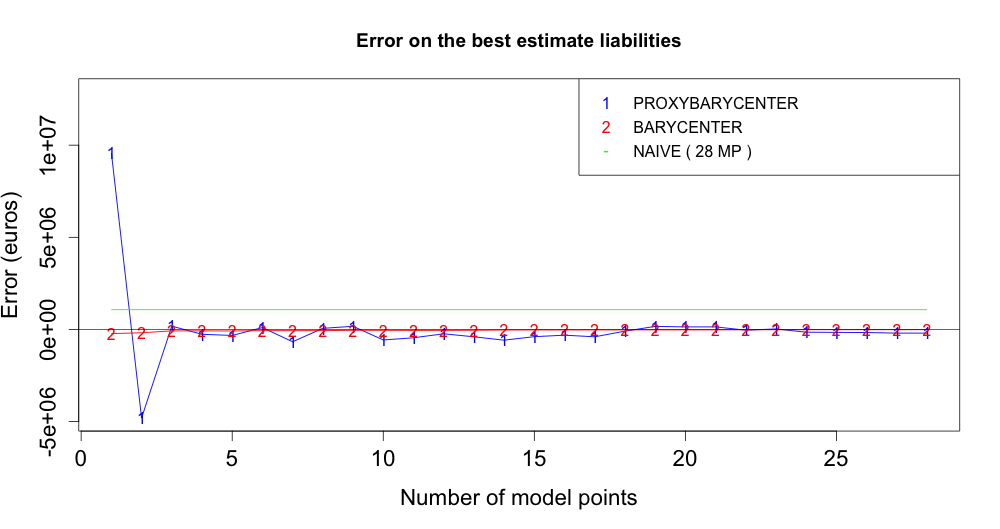
\includegraphics[width=15cm]{Chapitre6/EcartBel.png}
			\caption{Error on the BEL evaluation depending on the number of model points and the aggregation method}
			\label{BELError}
		\end{center}
	\end{figure}
\end{center}
\begin{center}
	\begin{figure}[ht!]
		\begin{center}
			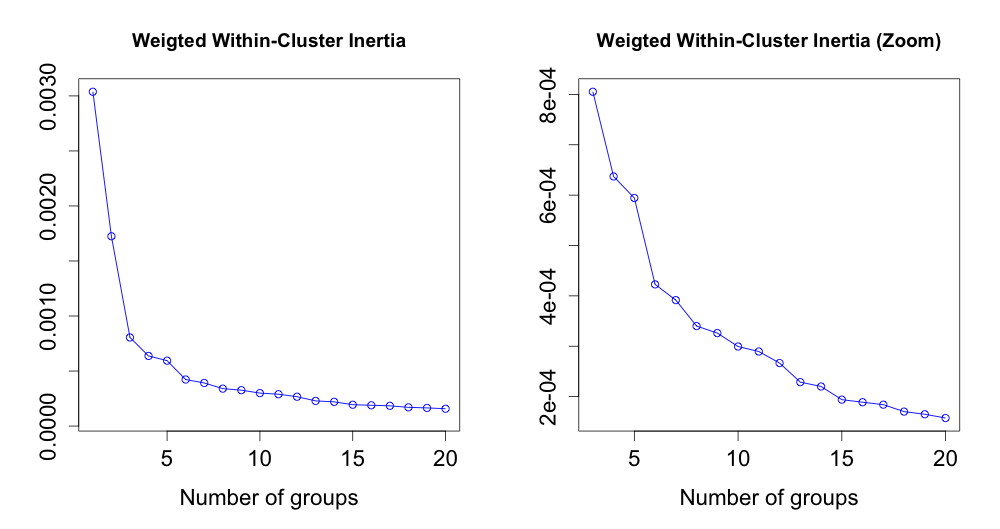
\includegraphics[width=15cm]{Chapitre6/WCSS.png}
			\caption{WWCI evolution depending on the number of clusters}
			\label{WCSS}
		\end{center}
	\end{figure}
\end{center}
This permits to compare the decreasing of WWCI in the data with the decreasing of WWCI within data uniformly distributed through space. The silhouette statistic has been introduced in \citet{KaRo90} and is defined, for each observation $i$, as 
\begin{equation}\label{Silhouette}
s(i)=\frac{b(i)-a(i)}{max\{a(i),b(i)\}},
\end{equation} 
where $a(i)$ is the average distance between $i$ and the others points in its cluster, and $b(i)$ is the average distance from $i$ to the data points in the nearest cluster besides its own.  A point is well clustered when $s(i)$ is large. The optimal number of clusters maximises the average of $s(i)$ over the data set. Figure \ref{PartitionIndex} displays the different indicators computed for every partition ranging from one to twenty groups. The different indicators seems to retain $3$ clusters (except for KL, that is maximized for $6$ clusters but still have a large value for $3$ clusters). Figure \ref{ClassifiedPTF} offers a visualization of the $3$-groups partition of the portfolio. Table \ref{3GroupsBELError} report the errors on the BEL, which have been normalized by its exact value and expressed in percentage. The presented methods outperform greatly the naive one with less model points. Our aggregation procedure does not only performed an accurate BEL evaluation but manages also to replicate the cash flows dynamics throughout the entire projection. Figure \ref{VAPChronical} shows the accuracy on the expected present value of the exiting cash flow associated with each projection year for the $3$-MP aggregated portfolio.
\begin{table}[ht!]
\centering
\begin{tabular}{|c|c|c|}
\hline
BEL error $\%$ &BEL error $\%$& BEL error $\%$\\
 BARYCENTER& PROXYBARYCENTER& NAIVE (28 MP)\\
\hline\hline
$-0.003$ $\%$&$0.007$ $\%$& $0.0412$ $\%$\\
\hline
\end{tabular}
\caption{Best estimate liabilities error with 3 model points depending on the aggregation method}
\label{3GroupsBELError}
\end{table}
\begin{center}
	\begin{figure}[ht!]
		\begin{center}
			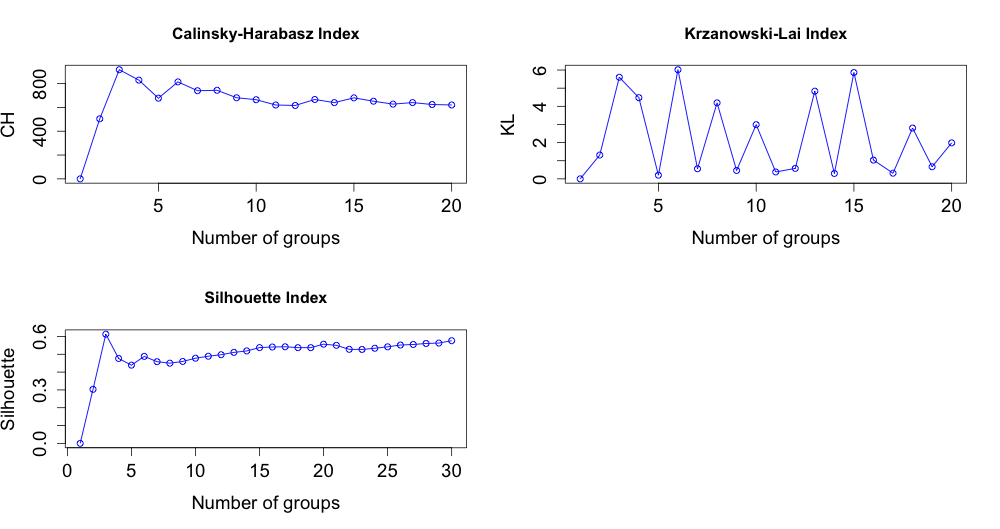
\includegraphics[width=15cm]{Chapitre6/PartintioningIndex.png}
			\caption{Partitionning quality indicators variations depending on the number of clusters}
			\label{PartitionIndex}
		\end{center}
	\end{figure}
\end{center}
From a practical point of view, the optimal number of clusters should be associated with a level of error chosen by the user. We did not manage to establish a clear link between WWCI and the error on the BEL evaluations. Maybe it does not exist and we need to define another indicator, instead of WWCI, that we can compute from the probabilities of surrender and that is more linked to the evaluation error. This a topic of current research. We may also add that the optimal number of clusters is not necessarily a problem that needs much thoughts from a practitionner point of view. The number of model points in the aggregated portfolio is often constrained by the capability of computers to deal with the valuation of large portfolios. The number of model points is then a parameter of the aggregation process. Another technical requirement is to take into account the different lines of business. Two life insurance products cannot be grouped together because they may have characteristics, besides their probabilities of surrender, that impact BEL computations. A solution is to allocate a number of model points for each line of business in proportion to their mathematical provision.  
\begin{center}
	\begin{figure}[ht!]
		\begin{center}
			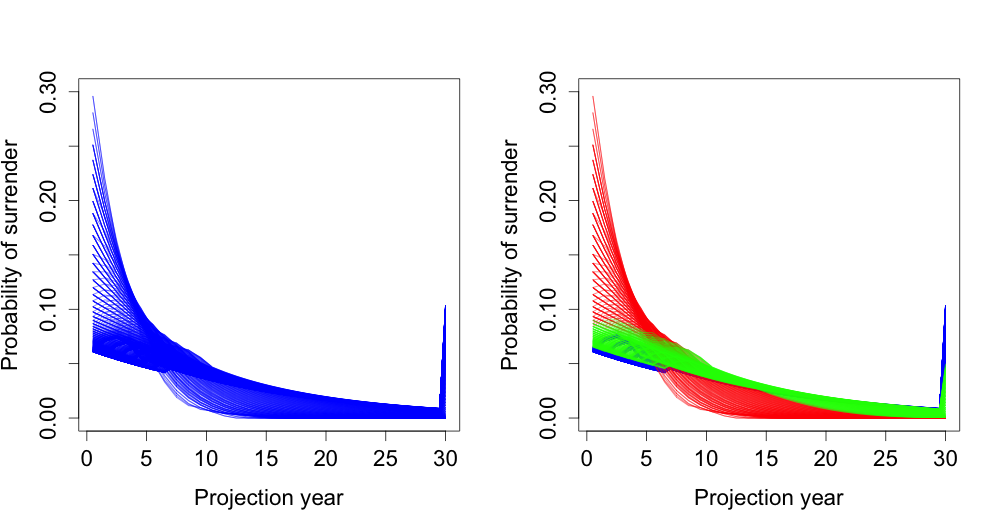
\includegraphics[width=15cm]{Chapitre6/TrajectoriesClassified.png}
			\caption{Portfolio visualization through its trajectories of surrender}
			\label{ClassifiedPTF}
		\end{center}
	\end{figure}
\end{center}
\begin{center}
	\begin{figure}[ht!]
		\begin{center}
			\includegraphics[width=15cm]{Chapitre6/VapChronical.png}
			\caption{Expected present value of surrender during the projection}
			\label{VAPChronical}
		\end{center}
	\end{figure}
\end{center}
\section{Conclusion}
The aggregation procedure permits a great computation time reduction that goes along with a limited loss of accuracy. The method is easy to understand and to implement as the statistical tools are available in most datamining softwares. The application may extend to the entire scope of life insurance business, and can be tailored to many cash flow projection model based on the general definition of best estimate liabilities given in the introduction. The production of aggregated portfolios can also be combined to optimization methods concerning economic scenarios. A reduction of the number of financial scenarios would permit to increase the number of model points. The optimal gain of accuracy would result from a trade-off between the number of model points and the number of financial scenarios.\\ 
This work represents the successful outcome of a Research and Development project in the industry. It is already implemented in AXA France, from a portfolio that contains millions of policies, the output is a portfolio of only a few thousands model points for a $0.005\%$ error on the BEL. It remains many rooms for improvement, especially at the partitioning level where distance other than euclidean might be better suited to quantify the distance between trajectories. The definition of an indicator that gives insight on the error resulting from the aggregation would be as well a great improvement. For instance, the computation of this indicator may provide an optimal number of model points allocated to each line of business and therefore the whole portfolio. 

\bibliographystyle{francaissc}
\bibliography{Chapitre6/BiblioChap6}